%TODO:  fix all figure numbers
%	make all code screenshots the same width



%% Use the hmcposter class with the clinic document-class option.
\documentclass[thesis]{hmcposter}
\usepackage{graphicx}
\usepackage{natbib}
\usepackage{booktabs}
\usepackage{subfig}
\usepackage{amsmath}
\usepackage{textcomp}
%\usepackage{url}
\usepackage{listings}

\usepackage{verbatim}

% Added by jeramey
\usepackage{caption}

% Added by cyrust
\usepackage{hyperref} % replaces url package


\posteryear{2017}

\title{Common Abstract Syntax Tree (AST) \\ for Automated Software Analysis \\ of Homework Assignments in Submitty}
\author{Elizabeth Dinella, Samuel Breese, Ana Milanova, and Barbara Cutler}


\classlogo{lgplogo2cm}
\classlogowidth{2in}

\raggedcolumns

%% Define the \BibTeX command, used in our example document.
\providecommand{\bibtex}{{\rmfamily B\kern-.05em%
    \textsc{i\kern-.025em b}\kern-.08em%
    T\kern-.1667em\lower.7ex\hbox{E}\kern-.125emX}}


\pagestyle{fancy}

\begin{document}

\begin{poster}

\section{Static Analysis}
Static analysis is a critical tool to ensure software security and dependability. In industry and academia, static analysis can be used to find potential bugs or design problems. On "Submitty", an open source homework server created at RPI, static analysis is used to ensure structural correctness on homework assignments. This functionality is used in RPI's Computer Science 1 (CSCI 1100) to automatically grade small in-lecture exercises. %Information beyond the textual output of the program would be valuable to assess knowledge. 
For example, consider the following assignment:
%For example, students in CS1 are typically asked to "re-write" a simple for loop using a while loop (figure a). In this exercise, the code containing a for loop, and the code containing a while loop would have the same textual output. However, it would be impractical for each assignment to be individually graded by the teaching staff. Static analysis tools are, in some cases, necessary to accurately asses student's progress.

%Additionally, static analysis is superior to simpler alternative methods. For example, running grep on the student's code could cause false positives. This situation is shown in figure c. Additionally, static analysis can be used to detect more complex structures such as class hierarchies and exception handling.

\begin{figure}
\begin{center}
\subfloat[Assignment: rewrite the above code using a while loop]{\label{fig:Initial Code}\fbox{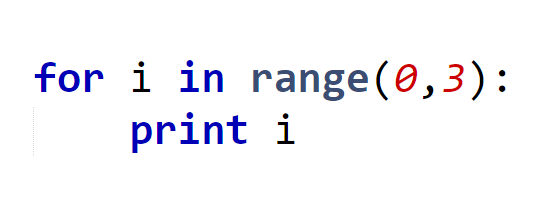
\includegraphics[width=4in]{initialCode}}}
\end{center}
\end{figure}

\begin{figure}
\begin{center}
\subfloat[Correct Student Rewrite]{\label{fig:Correct Student Rewrite}\fbox{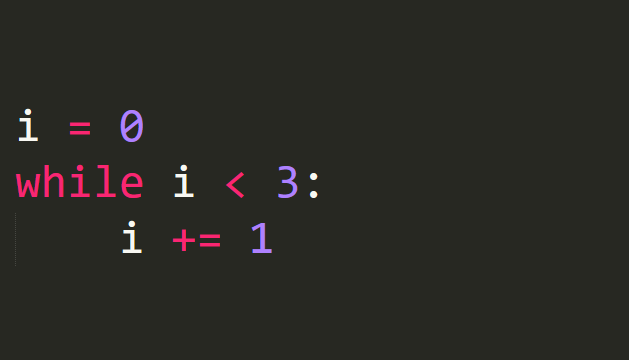
\includegraphics[width=4in]{studentRewrite}}}
\hspace{0.3in}
\subfloat[Incorrect Student Rewrite - creates a false positive when using tools like "grep"]{\label{fig:Correct Student Rewrite}\fbox{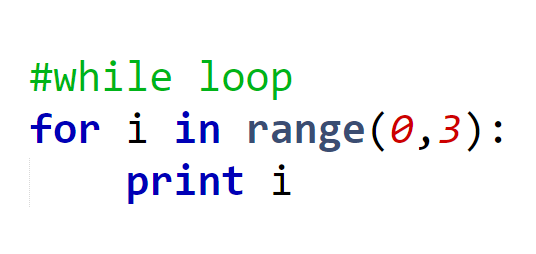
\includegraphics[width=4in]{studentRewriteError}}}
\end{center}
\end{figure}

In this example, all three segments of code would produce the same textual output. Static analysis is required to accurately assess student's progress and avoid false positives that occur in simpler alternatives.

\section{Motivation}
In this motivating example, a student in an introductory computer science course is tasked with the following assignment:
\\
\texttt{Create a loop in Python or C++ that prints all odd numbers between 1 and 10}
\\
%By only checking textual output, Submitty would not verify that the student's code actually includes any for loops. Without static analysis, a non-automated TA or instructor grade would be required. 
Consider the following correct solutions to this assignment:

%MAKE THE PYTHON SOLUTION VERTICALLY CENTERED
\begin{figure}
\begin{center}
\subfloat[Python Solution]{\label{fig:Python Solution}\fbox{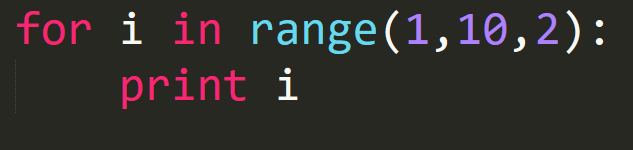
\includegraphics[width=4in]{pythonassign}}}
\hspace{0.4in}
\subfloat[C++ Solution]{\label{fig:Python Solution}\fbox{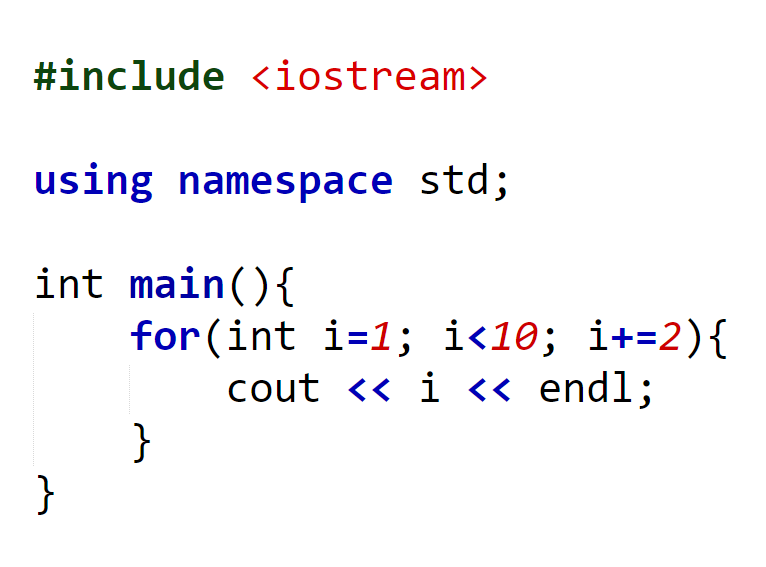
\includegraphics[width=4in]{c++assign}}}
\end{center}
\end{figure}

Static analysis tools have been requested for other porgramming languages. To implement a simple static analysis tool for while/for loop detection for C++ and Java, the entire framework and the tool must be re-written in each language. 
%This requires a large code base that depends upon extensive development each time a new language is used.
Our project provides an alternative by enabling the re-use of static analysis tools across multiple languages.

%It may seem excessive to create an entire new framework for each language, but it is necessary due to the uniqueness of each languages intermediate code representation. During parsing and semantic analysis, an Abstract Syntax Tree (AST) is created to represent code structure. In each language, there are drastic AST differences. 

%

\columnbreak

\section{Introduction}
Our project builds a Common Abstract Syntax Tree (Common AST) which captures the structural similarity of the different languages and covers the use cases for static analysis on Submitty. The Common AST is extracted from C++ and Python code and is stored in a standardized XML format. 
%Extraction occurs using Clang/LLVM AST matchers and the Python AST module. 
This framework allows a simple process for adding new static analysis tools for different programming languages.
The common AST captures relevant structures from Python and C++:

\vspace{0.3in}
\begin{figure}
\begin{center}
\subfloat[Common AST]{\label{fig:Common AST}\fbox{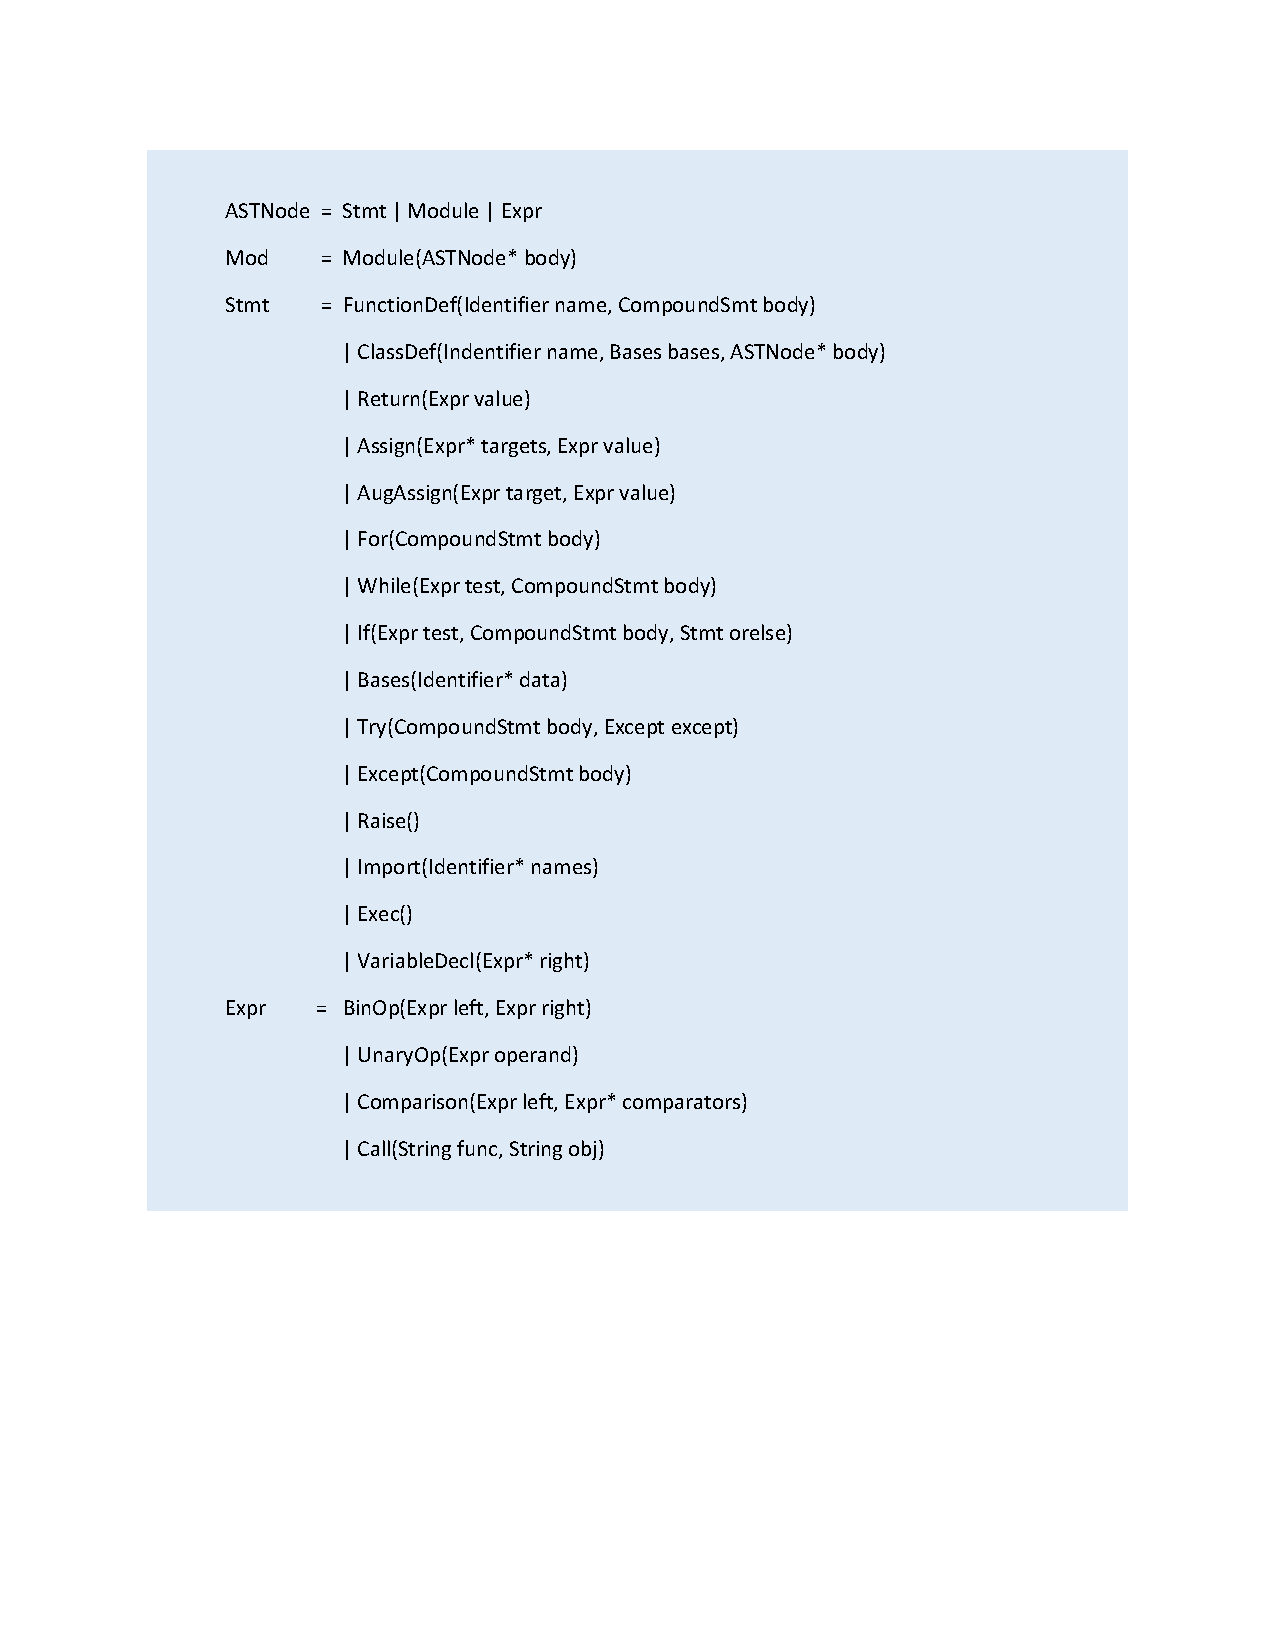
\includegraphics[width=10in]{AST}}}
%\hspace{0.3in}%
\end{center}
\end{figure}
\vspace{0.3in}

%TALK ABOUT HOW MY TOOL WOULD BE IDEA FOR THIS 
\section{Standardized XML Format}

We begin with a syntax directed translation process. In this phase, we translate the original AST into a standardized XML format that represents the Common AST.
\vspace{0.5in}
%In order to translate the original AST into the standardized XML format we:
\begin{itemize}
\item Remove all information that is irrelevant to the Submitty use cases 
\item output a sequence of tokens in the following format: \texttt{<node, level>}
	\begin{itemize}
	\item \texttt{node} is the name of the corresponding structure in the source code. It may represent any of the productions in the common grammar (figure d).
	\item \texttt{level} represents the depth in the syntax tree. %For example, in figure d, the while loop is a child of the outer python module. So, the while loop has a level of 2. The while loop holds its body as a child. The body contains one child, the augmented assignment of p. So, "p++" has a level of 4, and the token reads: \texttt{<augAssign,4>}
	\end{itemize}
\end{itemize}
\vspace{0.5in}
%
%\begin{figure}
%\begin{center}
%\subfloat[Level Example]{\label{fig:Level Example}\fbox{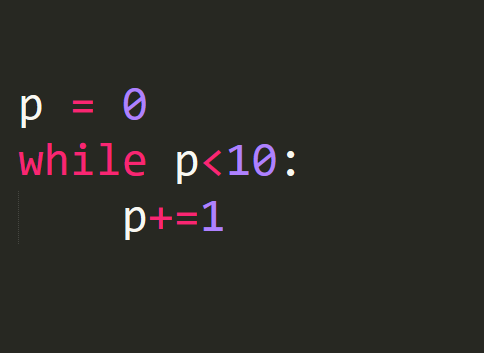
\includegraphics[width=4in]{levelExample}}}
%\end{center}
%\end{figure}

\columnbreak

This format is created using third party libraries that allow users to process the abstract syntax trees of external programs. For C++, Clang/LLVM AST Matchers are used to traverse the AST of an input file. During traversal, when a node relevant to the use cases is found, a token is created and printed to an output file. A similar process occurs for Python using the Python AST library.

Figures e and f show the standardized XML output from the two assignment solutions.

\begin{figure}
\begin{center}
\subfloat[Python Standardized XML corresponding to figure d]{\label{fig:Python Standardized XML}\fbox{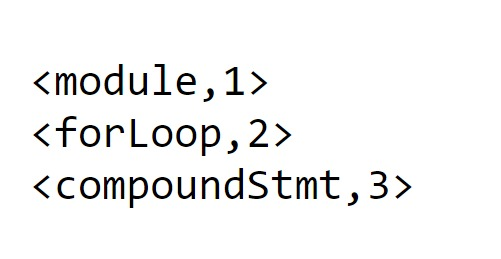
\includegraphics[width=4in]{pythonXML}}}
\hspace{0.4in}
\subfloat[C++ Standardized XML corresponding to figure e]{\label{fig:C++ Standardized XML}\fbox{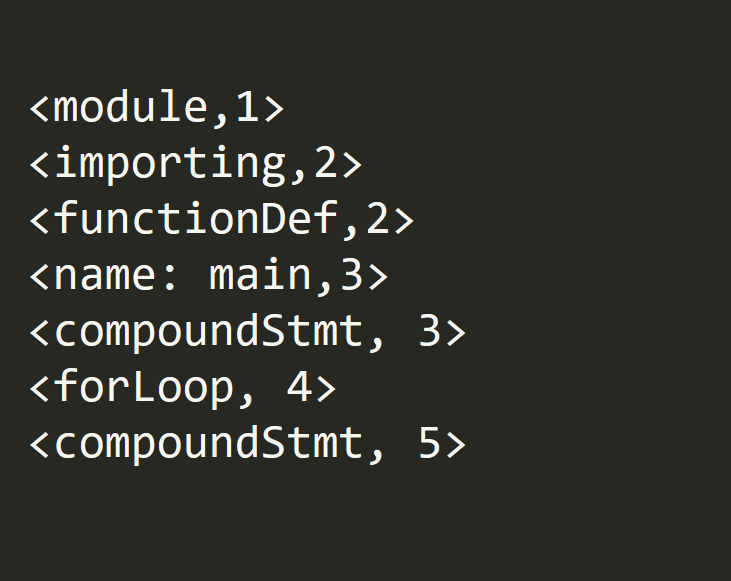
\includegraphics[width=4in]{C++XML}}}
\end{center}
\end{figure}


\section{Recursive Descent Parser}
The standardized XML output contains the common AST structure. In this phase, we parse the XML into a Common AST in memory.
%In this phase, tokens from the previous phase are taken as input. The tokens are compared to the grammar and a syntax tree is generated. 
vspace{0.5in}
To recursively create a Common AST in a depth first top-down order we:
\begin{itemize}
\item Take the standardized XML output from the first step as input
\item At each level of the recursion, the token in the AST is dispatched to an appropriate processing function based on the node type
	\begin{itemize}
	\item There is a processing function for each production that follows the grammar.
		%For example, the production for a FunctionDef shown in figure d, has an Identifier for its name and a CompoundStmt for its body. The processing function for a FunctionDef is shown in figure j. In each processing function, a class of type corresponding to the input token is created. 
	The member variables are initialized recursively. In this way, a node's children are stored in a has-a pointer relationship. 
	\end{itemize}
\end{itemize}

\vspace{0.5in}

\begin{figure}
\begin{center}
\subfloat[FunctionDef Processing Function]{\label{fig:FunctionDef Processing Function}\fbox{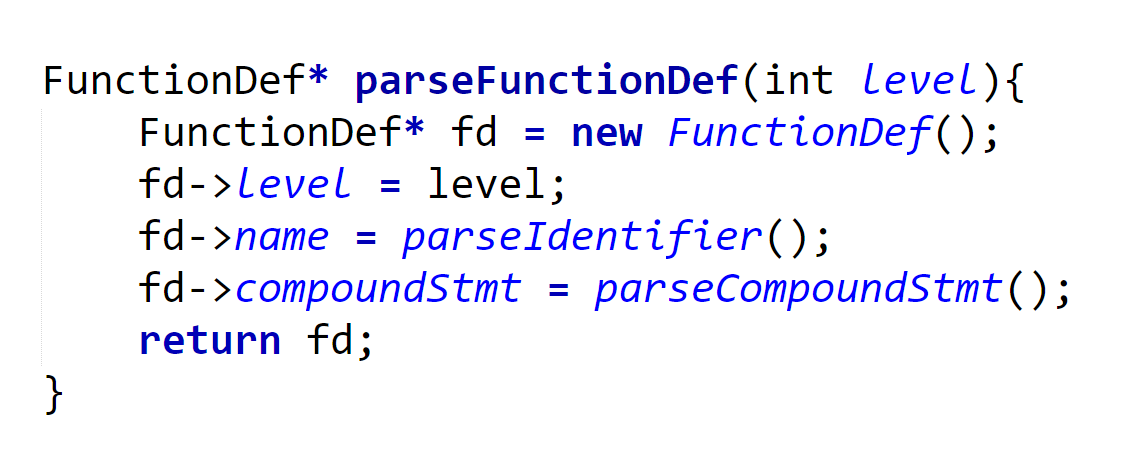
\includegraphics[width=10in]{functionDef}}}
\end{center}
\end{figure}

\columnbreak
\section{Use Cases}
Use cases suggested by Submitty instructors:
\begin{itemize}

%
%\item{Detecting or counting if statements}
%	\begin{itemize}
%		\item {Nested if statements}
%		\item {Dangling else cases}
%	\end{itemize}

\item{Detecting or counting for/while loops and if statements; nested loops and crude complexity analysis}
\item{Detecting language specific keywords such as "goto", "malloc", "auto", etc}	
\item{Detecting member function calls from an outside class such as "vector.erase()"}
\item{Counting number of calls to a given function}
\item{Detecting exceptions and ensuring a corresponding handler}
\item{Detecting "code clones" between different languages}
\item{Detecting is-a (inheritance) and has-a (composition) relationships; detecting design patterns}
\end{itemize}

\section{Ongoing Work}
\begin{itemize}
\item{Implementation of use cases}
\item{Large scale testing on RPI Data Structures (CS 1200) and RPI Computer Science 1 (CS 1100) assignments}
\item{Possible extension of framework to include Java}
\end{itemize}


\section{Related Publications}
\begin{itemize}
\item \textit{Using Static Analysis for Automated Assignment Grading in Introductory Programming Classes}, Breese, Milanova, Cutler, SIGCSE 2017 Static Analysis Poster 
\item \textit{User Experience and Feedback on the RPI Homework Submission Server}, Wong, Sihsobhon, Lindquist, Peveler, Cutler, Breese, Tran, Jung, and Shaw, SIGCSE 2016 Poster 
\item \textit{A Flexible Late Day Policy Reduces Stress and Improves Learning} Tyler, Peveler, and Cutler,
SIGCSE 2017 Poster
\item \textit{Submitty: An Open Source, Highly Configurable Platform for Grading of Programming Assignments}, Peveler, Tyler, Breese, Cutler, and Milanova, SIGCSE 2017 Demo Presentation
\end{itemize}

\section{Acknowledgments}
\begin{itemize}
    \item Red Hat Software
    \item Rensselaer Center for Open Source (RCOS)
    \item \url{http://submitty.org/}
    \item \url{https://github.com/Submitty/Submitty}
\end{itemize}

\end{poster}

\end{document}

